%\chapter{det-comp}


%%%%%%%%%%%%%%%%%%%%%%%%%%%%%%%%%%%%%%%%%%%%%%
%\section{Anode Plane Assemblies}

%%%%%%%%%%%%%%%%%%%%%%%%%%%%%%%%%%%%%%%%%%%%%%
%\section{Cathode Plane Assemblies}

%%%%%%%%%%%%%%%%%%%%%%%%%%%%%%%%%%%%%%%%%%%%%%
\section{Field Cage (FC)}
\label{detcompsec-fc}
%%%%%%%%%%%%%%%%%%%%%%%%%
%\subsection{Scope, Requirements and Design Parameters}
\subsection{Scope and requirements} 

In the TPC, each pair of facing cathode and anode planes form an electron-drift region. A field
cage (FC) must completely surround the four open sides of this region to provide the necessary boundary
conditions to ensure a uniform electric field within, unaffected by the presence of the cryostat walls.  The scope of the FC includes:

\begin{itemize}
\item six top FC assemblies;
\item six bottom FC assemblies; and
\item four end-wall panels, each of which consist of four (side) assemblies.
\end{itemize}

Each assembly is made up of
\begin{itemize}
\item parallel metallic profiles;
\item a resistive divider chain that interconnects the parallel metal profiles  to provide voltage step-down;
\item FR4 I-beams that form a support structure for the top and bottom assemblies; and
\item ground planes (GP) for the top and bottom assemblies, six GP panels per FC module.
\end{itemize}

In addition, the FC assemblies include FR4 pieces to make the mechanical connections to the CPA and APAs.
One end-wall assembly is specially configured to accommodate the
cylindrical beam plug, which displaces the LAr in the region where the beam enters the cryostat.

The FC is required to:
\begin{itemize}
\item provide the nominal drift field of 500\,V/cm;
\item withstand $-$180\,kV near the cathode;
\item define the drift distance between the APAs and CPAs to <1\,cm;
\item limit the electric field in the LAr volume to under 30\,kV/cm;
\item miminize the peak energy transfer in case of a HV discharge anywhere on the field cage or cathode;
\item provide redundancy in the resistor divider chain;
\item maintain the divider current much greater than the ionization current in the TPC drift cell, yet less than the power supply current limit when all dividers are connected in parallel;
\item be modular in form such that they can be easily installed in the cryostat;
\item provide support for the beam plug; 
\item support a 200-lb. person standing on the support beam of the bottom FC module; and
\item prevent any trapped volume of liquid.
\end{itemize}

%%%%%%%%%%%%%%%%%%%%%%%%%
\subsection{Mechanical design}

The FC has six top and six bottom FC assemblies, arranged in sets of three along each horizontal boundary of the two drift regions. It has 
four end-wall panels (each made up of four end-wall assemblies), one covering each vertical boundary of the two drift regions, shown in Figures~\ref{fig:fc-overview} and~\ref{fig:fc-endwall_module}.
Each endwall panel consists of four assemblies in ``landscape'' orientation, stacked vertically.
FC assemblies are constructed from pultruded G10 I-beams and box beams that support extruded field-shaping aluminum profiles. The support structure for each of the top and bottom FC assemblies consists of two main I-beams that are 3.6~m long, and three cross I-beams that brace the main I-beams for structural stability. The main I-beams have cutouts to hold the field-shaping profiles. 

\begin{cdrfigure}[An end-wall field cage assembly]{fc-endwall_module}{A view of an end-wall field cage assembly. An end-wall panel consists of a stack of four of these assemblies (each in landscape orientation).}
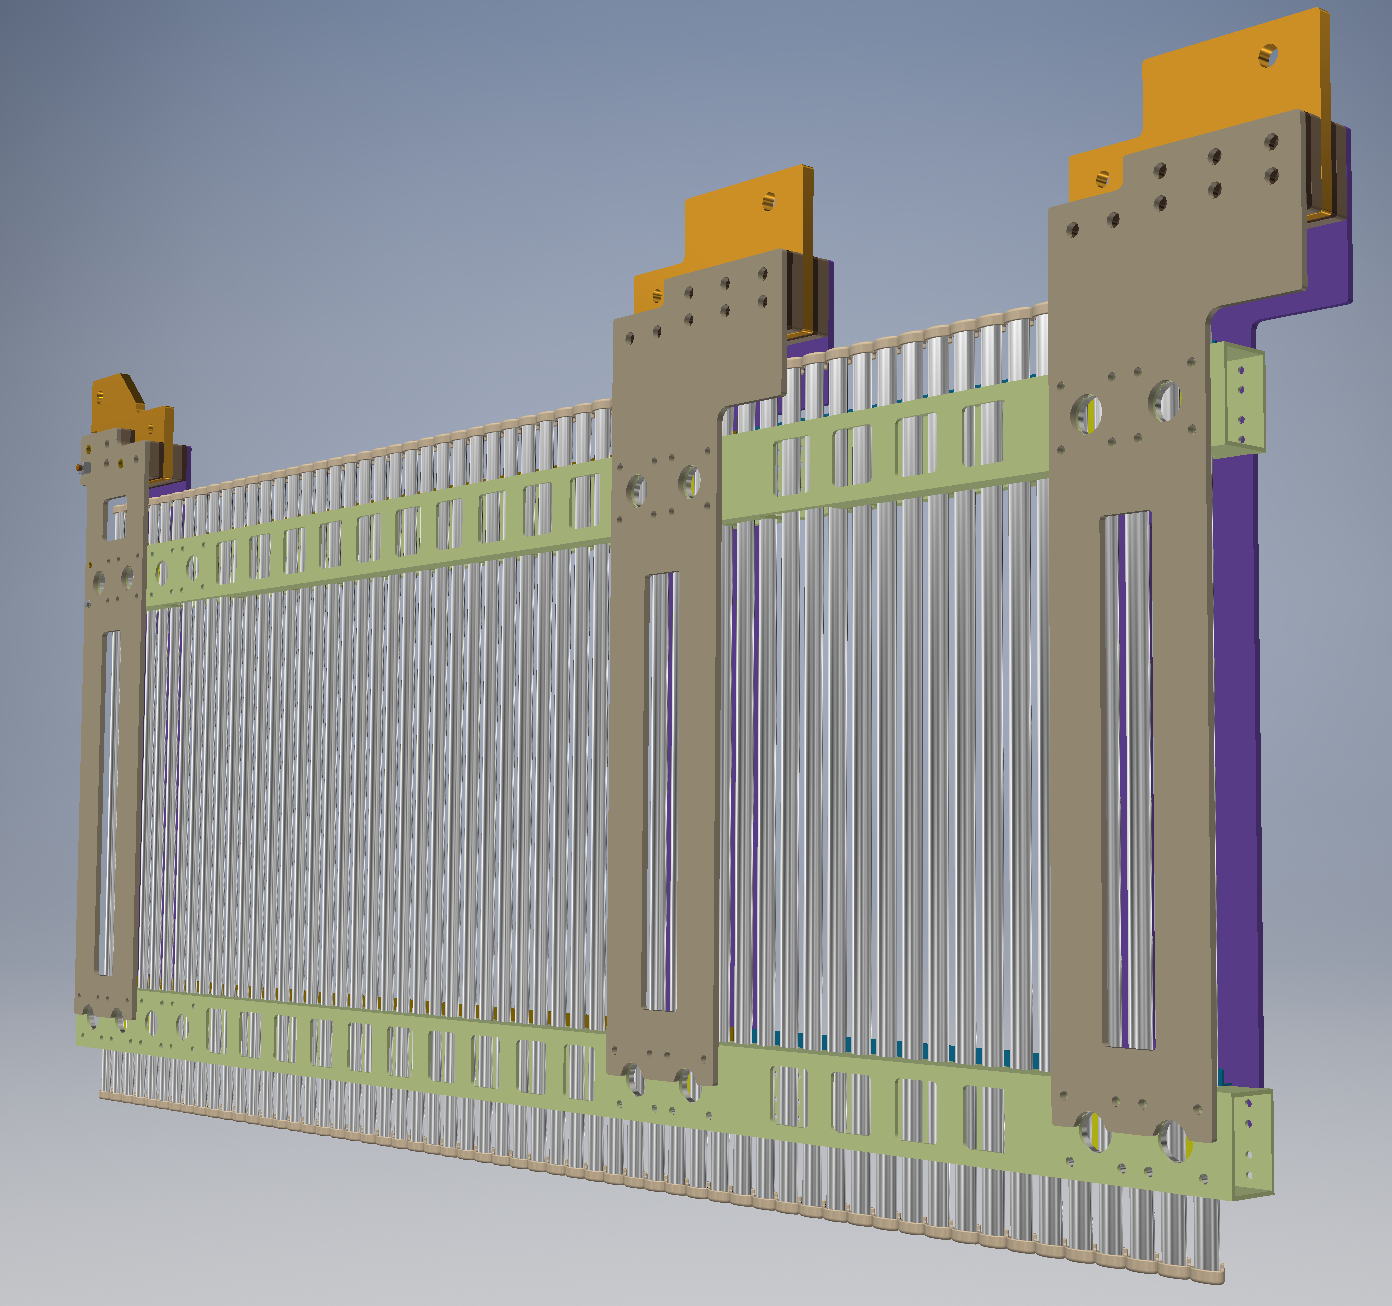
\includegraphics[width=0.6\linewidth]{tpc_fc_endwall_module.png}
\end{cdrfigure}

Aside from the profiles themselves, the nuts and bolts holding them, and the ground plane panels, all FC components are made of insulating material. The material selected for these structural components is fiberglass-reinforced plastic (FRP), which prevents binding when the structure is at cryogenic temperatures. The ground plane panels are made of stainless steel. 

The inward-facing side of the ground planes are approximately 20~cm away from the top of the field-shaping profiles, mounted at this fixed distance % from the field shaping profiles 
by standoffs. Figure~\ref{fig:fc-with-ground-planes} shows a set of ground planes situated over the I-beams and cross beams attached to a FC assembly.

\begin{cdrfigure}[The field cage with ground planes]{fc-with-ground-planes}{The field cage with ground planes}
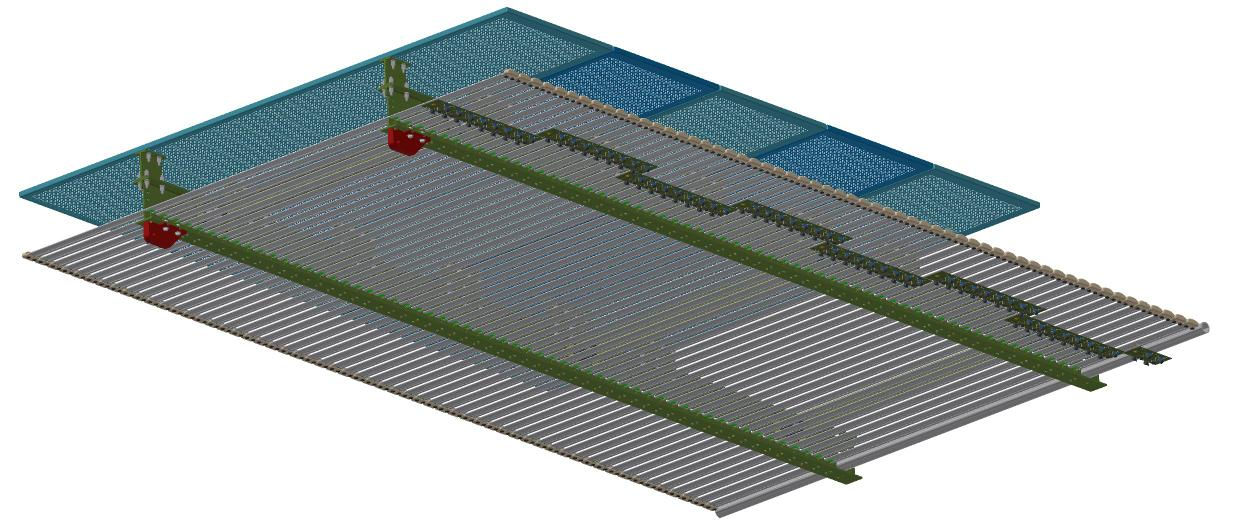
\includegraphics[width=0.8\linewidth]{fc-with-ground-planes}
\end{cdrfigure}

The parallel metal profiles in each FC assembly 
 are interconnected by a resistive divider chain, and supported by the FRP beams that span the drift distance.  Between adjacent field cage assemblies, however,  
the metal profiles are neither mechanically nor electrically connected. Gaps between assemblies that range from a few millimeters to a few centimeters are designed into the TPC assembly to ensure sufficient clearance for the installation.  The electrical isolation between the field cage modules minimizes the peak energy dump in case of a HV discharge.


%%%%%%%%%%%%%%%%%%%%%%%%%
\subsection{Electrical design}

Given a large standoff distance between the FC and the grounded cryostat wall, it is relatively easy to design a FC that meets the 30-kV/cm electric field limit with 180-kV bias.  However, as this distance is reduced to increase the active detector volume, the design becomes more challenging.  Optimizing the active detector volume requires the use of electrodes with low profiles, rounded edges, no trapped volumes, and low cost.  Fortunately, several commercially available roll-formed metal profiles were studied and appear to meet these requirements. 

Figure~\ref{fig:fc-schematic} is a schematic of the electrical design of  the CPA and a top/bottom field cage module pair.

\begin{cdrfigure}[Field cage schematic diagram]{fc-schematic}{A schematic diagram of the CPA and a top/bottom field cage module pair}
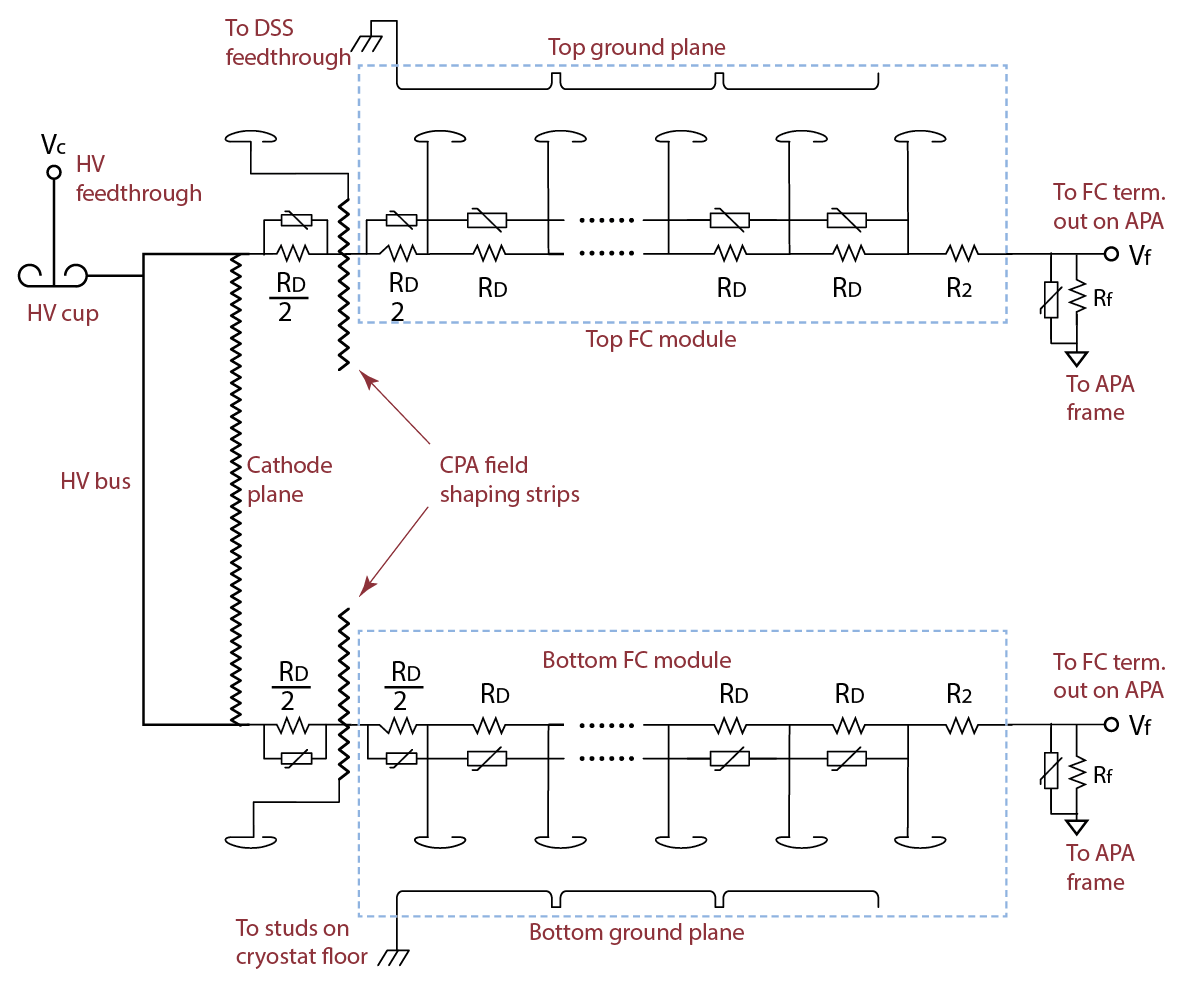
\includegraphics[width=0.8\linewidth]{tpc_fc_schematic.png}
\end{cdrfigure}

%%%%%%%%%%%%%%%%%%%%%%%%%
\subsection{Top/bottom FC assemblies and GP modules}

In order to confine the electric field in the active LAr region, a grounded metallic plane is installed between the upper FC assemblies and the liquid-gas interface, and also between the lower FC assemblies and the bottom of the cryostat. 
Each of the six top FC assemblies has six ground plane (GP) panels attached to it, aligned 
along their long %(2,318-mm) 
(2.3-m) dimension. The GPs are connected to the FC I-beam 
with additional 
G10 support pieces that are also used to connect adjoining GP panels. 
Figure~\ref{fig:fc-panel-endwall-frame} shows the frame of a top/bottom FC assembly and 
Figure~\ref{fig:fc_full} shows a 3D model of a fully assembled FC module with attached GP panels.

\begin{cdrfigure}[Top/bottom FC panel with endwall frame]{fc-panel-endwall-frame}{A top/bottom FC assembly with the frame}
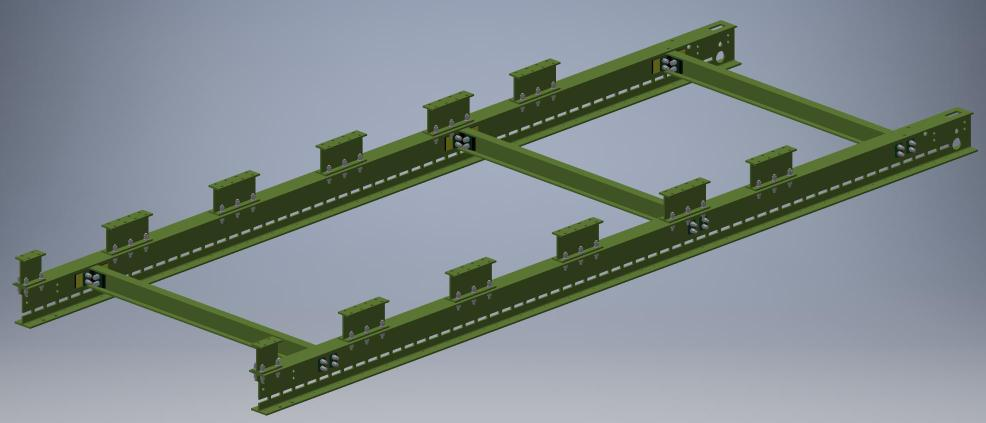
\includegraphics[width=0.8\linewidth]{fc-panel-endwall-frame}
\end{cdrfigure}

\begin{cdrfigure}[3D model of one fully assembled FC+GP module]{fc_full}{3D model of one fully assembled FC+GP module}
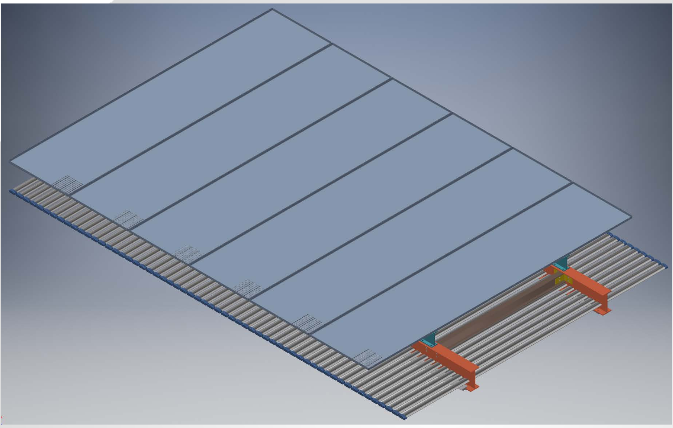
\includegraphics[width=0.8\linewidth]{tpc_topFC.png}
\end{cdrfigure}

The electrical connections between consecutive panels are to be made 
with either metallic screws (using holes on the planes edges) or looser connections, e.g., copper strips, that better adapt to the shrinking of the structure during cooldown. 
The GP panels are connected directly to the detector ground, referenced from the top of the cryostat.


In addition to the six primary GP panels attached to the the top FC modules,
\begin{itemize}
\item Smaller panels are to be connected to the modules on one side of the CPA so that, once in position, they 
cover the CPA frame. Their dimensions are 
still to be defined, depending on the final design of the CPA hanging scheme. These pieces will also connect to the top FC modules covering the opposite drift region, once in their final position.
\item An additional 
set of small panels is installed on the outer top FC modules of the FC to extend the GP coverage over the end-wall FC 
assemblies to further constrain the electric field in these regions. A FEA 
shows that the optimized overhang distance is 20~cm, provided that the surface of the LAr is 40\,mm above the GP. 
In this configuration, the maximal residual field is of the order of 13~kV/cm, with no greater than 1\,kV/cm fields in the gass ullage at the top of the cryostat.
\end{itemize}

%%%%%%%%%%%%
\subsection{Interfaces to other TPC components}

\subsubsection{FC to CPA}

On the top and bottom of the TPC, hinges connect each FC module to two CPA columns. These hinges allow the FC modules to be pre-attached to the CPAs during installation, preventing accidental damage to the APA wire planes when FC modules are raised and connected to the APAs.

The end-wall FC assemblies are hung from the CPA and APA support rails.  There is no strong mechanical coupling 
between the end-wall FC assemblies and the CPAs or APAs. However, the end-wall FC module resistive divider chains do have an electrical connection to the HV bus on the CPA plane.

\begin{cdrfigure}[CPA to field cage connection]{cpa-fc-connection}{A top field cage module (grey) connected to two CPA modules (brown)}
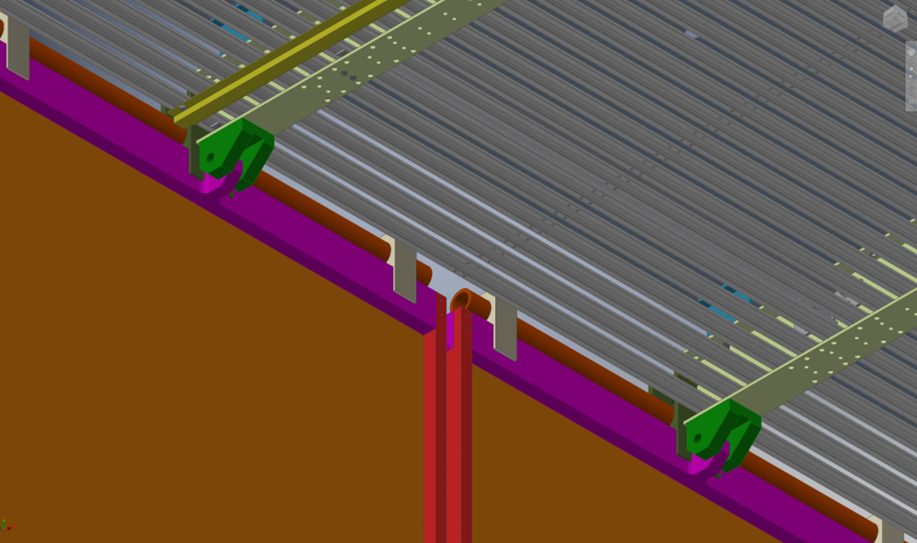
\includegraphics[width=0.8\linewidth]{tpc_fc_cpa_connection.png}
\end{cdrfigure}


%%%%%%%%%%%%
\subsubsection{FC to APA}

The I-beams of the top/bottom FC modules are designed to be latched onto  mating brackets on the APAs.  
In addition to the mechanical connection, the ground side of the divider chain must be connected to the APA's frame ground.  There is also an electrical connection between the FC module resistor divider chains, and ground is referenced from the APA frame.

%%%%%%%%%%%%
\subsubsection{FC to beam plug}
\label{subsec:fc-beamplug}

%The beam plug is installed between the field cage and primary membrane where the charged particle beam enters the cryostat. Its main function is to displace about 45 cm of passive LAr layer in that region to allow the particle beam to enter the active TPC region with minimal upstream material interactions. 

%To minimize the material interactions of the particle beam in the cryostat upstream of the TPC, a volume of LAr along the beam path (between the cryostat membrane and the FC) is displaced, and replaced by a less dense volume of dry nitrogen gas. The gas is contained within the \textit{beam plug}, a cylindrical glass-fiber composite pressure vessel, about 50\,cm in length and 22\,cm in diameter.


The LAr-displacement beam plug, a cylindrical glass-fiber composite pressure vessel, about 50\,cm in length and 22\,cm in diameter, is filled with nitrogen gas via a stainless steel line that extends to the top of the cryostat. It is illustrated in Figure~\ref{fig:beamplug}.
A pressure relief valve (or burst disk) is installed on the nitrogen fill line on the top of the cryostat (externally) to ensure the pressure inside the beam plug does not exceed the safety level of 25\,psi. A component-level view of the beam plug is shown in Figure~\ref{fig:beamplug_components}.  The beam plug is secured to the FC support structure as described in Section~\ref{subsec:fc-beamplug}. The front portion of the beam plug extends  5\,cm into the active region of the TPC  through an opening in the FC. The FC support is designed with sufficient strength and stiffness to support the weight of the beam plug before filling, while it is suspended in air.  When the cryostat is filled with LAr, the beam plug is roughly neutrally buoyant.  The total internal volume of the beam plug is about 16 liters. 

%As illustrated in Figure~\ref{fig:beamplug}, it is a cylidrical glass-fiber composite pressure vessel about 50cm in length and  22cm in diameter. It is filled with dry nitrogen gas via a stainless steel line that extends to the top of the cryostat. The pressure inside the beam plug is maintained externally up to 25 psi from room to LAr temperatures. A pressure relief valve (or burst disk) is installed on the nitrogen fill line on the top of the cryostat (externally) to ensure the pressure inside the beam plug does not exceed the safety level. The component-level view of the beam plug is shown in Figure~\ref{fig:beamplug_components}.  The beam plug is secured to the field cage support structure as described in Section~\ref{subsec:fc-beamplug}. The front portion of the beam plug extends 5~cm beyond the profiles to inside the active region of the TPC through an opening on the field cage. The field cage support is designed with sufficient strength and stiffness to support the weight of the beam plug while it is suspended in air.  When the cryostat is filled with LAr, the beam plug is roughly neutrally buoyant.  The total internal volume of the beam plug is about 16 liters. 

The requirements on the acceptable leak rate is between $7.8\times 10^{-5}$ scc/s and $15.6\times 10^{-5}$ scc/s. This is very conservative and is roughly equivalent to leaking  15\% of the nitrogen in the beam plug over the course of a year.
  In the worst-case scenario in which all the nitrogen in the beam plug leaks into the LAr cryostat, the increase in concentration is about 0.1\,ppm, which is still a factor of 10 below the maximum acceptable level, as specified by light detection requirements.
  \fixme{need some reference with details for this requirement}
  At nominal operation, the voltage difference across the beam plug (between the first and the last grading ring) is 165\,kV. 

    To minimize risk of electrical discharges, the beam plug is divided into sections, each of which is bonded to stainless steel conductive grading rings. The seven grading rings are connected in series with two parallel paths of resistor chains. The ring closest to the FC is electrically connected to one of the FC profiles. 
  The ring nearest the cryostat wall is grounded to the cryostat inner membrane via a short grounding cable. 
  The type and value of the resistor is still under evaluation.
  \fixme{still?}
  A likely candidate is the high-voltage Super Mox 15-G$\Omega$ resistor by OHMITE. The maximum total power dissipated by the resistor chain is about 0.6\,W.


\begin{cdrfigure}[Beam plug]{beamplug}{The beam plug is a  composite pressure vessel filled with dry nitrogen gas. The vessel is about 50\,cm in length and about 22\,cm in diameter. The pressure vessel is divided into sections with each section bonded to a stainless steel grading ring. The grading rings are connected by two parallel paths of resistor chain.}
  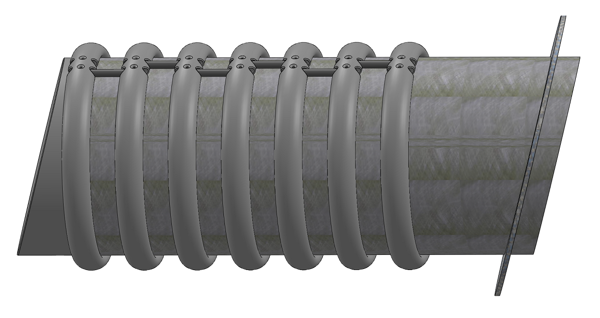
\includegraphics[width=0.6\textwidth]{beamplug.png}
\end{cdrfigure}

\begin{cdrfigure}[Beam plug component-level view]{beamplug_components}{Component-level view of the beam plug showing alternating electrode and composite ring structure.}
  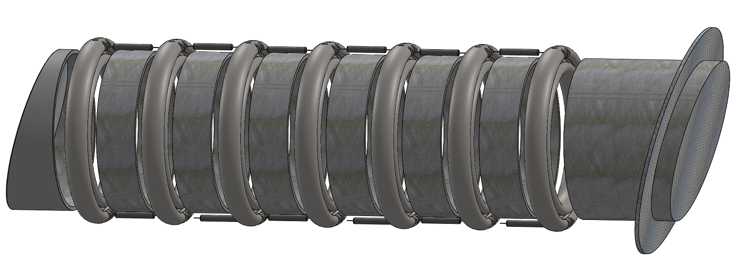
\includegraphics[width=0.7\textwidth]{beamplug_components.png}
\end{cdrfigure}

The metal electrode rings are spaced at regular intervals and interspersed with composite tube sections. The shape of the rings has been designed to minimize high electric field corners. The results of the field calculations are shown in Figures~\ref{fig:beamplug_ring1} and~\ref{fig:beamplug_ring2}. The average field in the vicinity of the beam plug is about 4.4\,kV/cm. The maximum field of 15.7\,kV/cm is on the electrode ring surface. In all regions the field is well below the 30-kV/cm limit.
\fixme{citation to doc describing limit would be good}

\begin{cdrfigure}[Beam plug electrodes]{beamplug_ring1}{Electric field calculation of the electrode ring design. The average field in the beam plug region is about 4.4 kV/cm. The maximum field of 15.7\,kV/cm is on the electrode ring surface. }
  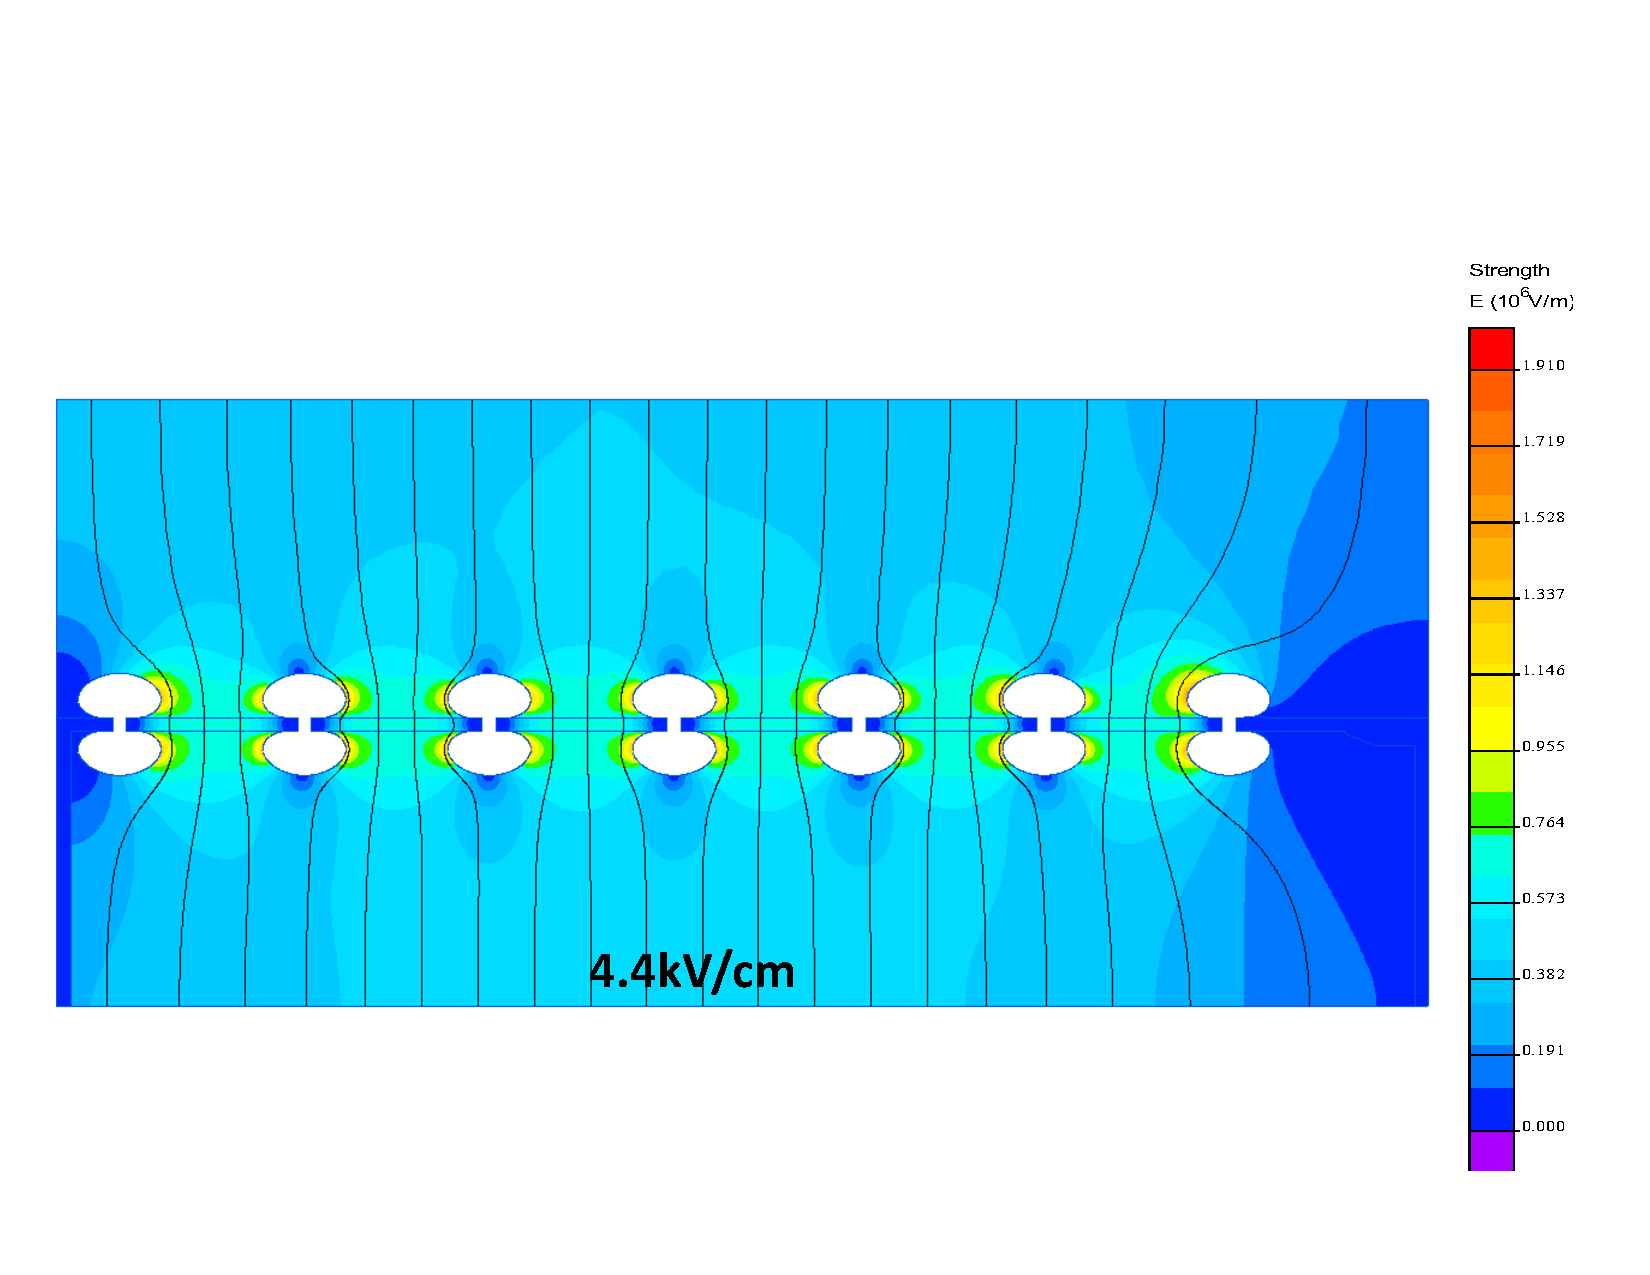
\includegraphics[width=0.85\textwidth]{beamplug_ring1.pdf}
\end{cdrfigure}

\begin{cdrfigure}[Beam plug electrode]{beamplug_ring2}{Electric field calculation near the vicinity of the electrode. The shape of the ring minimizes the high field region near the joints between the electrode, LAr, and composite shell. The field is well below the 30-kV/cm limit in all regions.}
  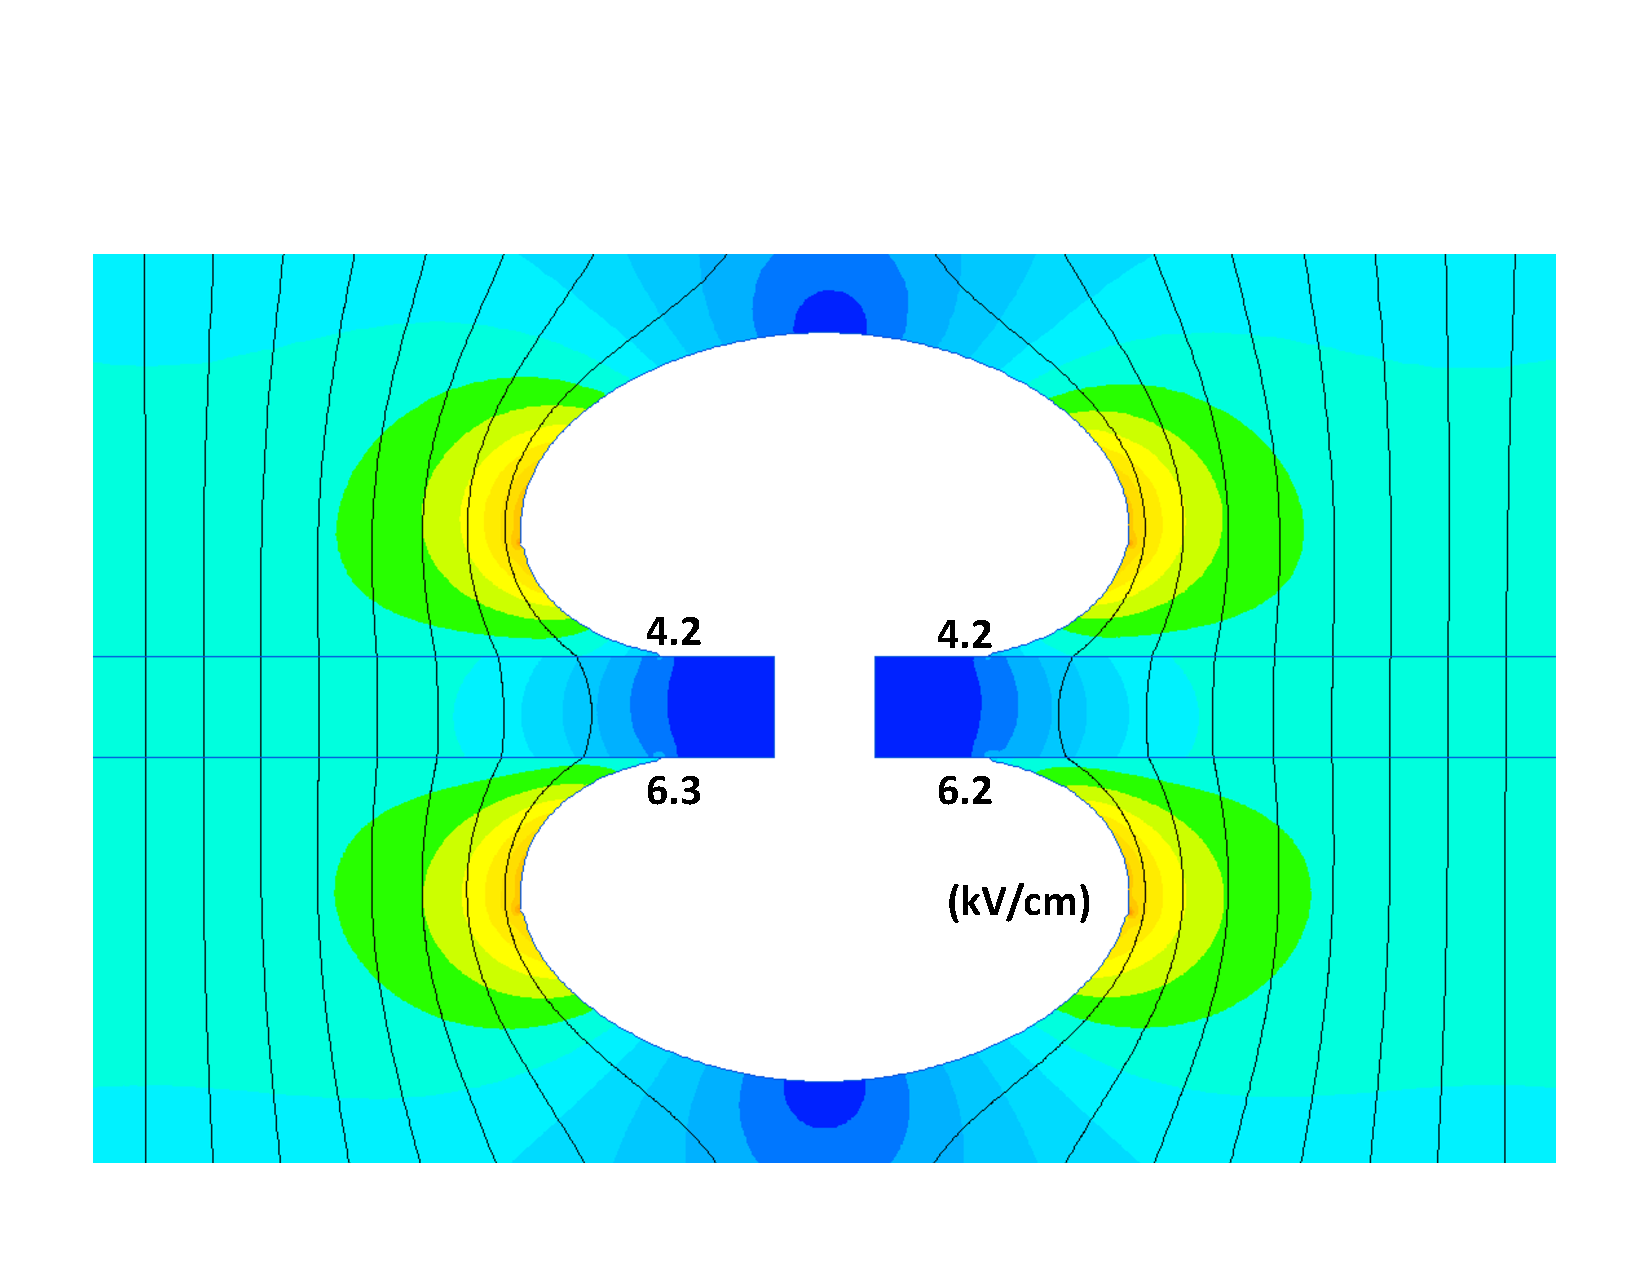
\includegraphics[width=0.5\textwidth]{beamplug_ring2.pdf}
\end{cdrfigure}

The beam plug is mounted onto one of the field cage support structures as shown in Figures~\ref{fig:beamplug-fc} and~\ref{fig:beamplug-fc2}. 
\begin{cdrfigure}[Beam plug to CPA connection]{beamplug-fc}{Beam plug to field cage interface.}
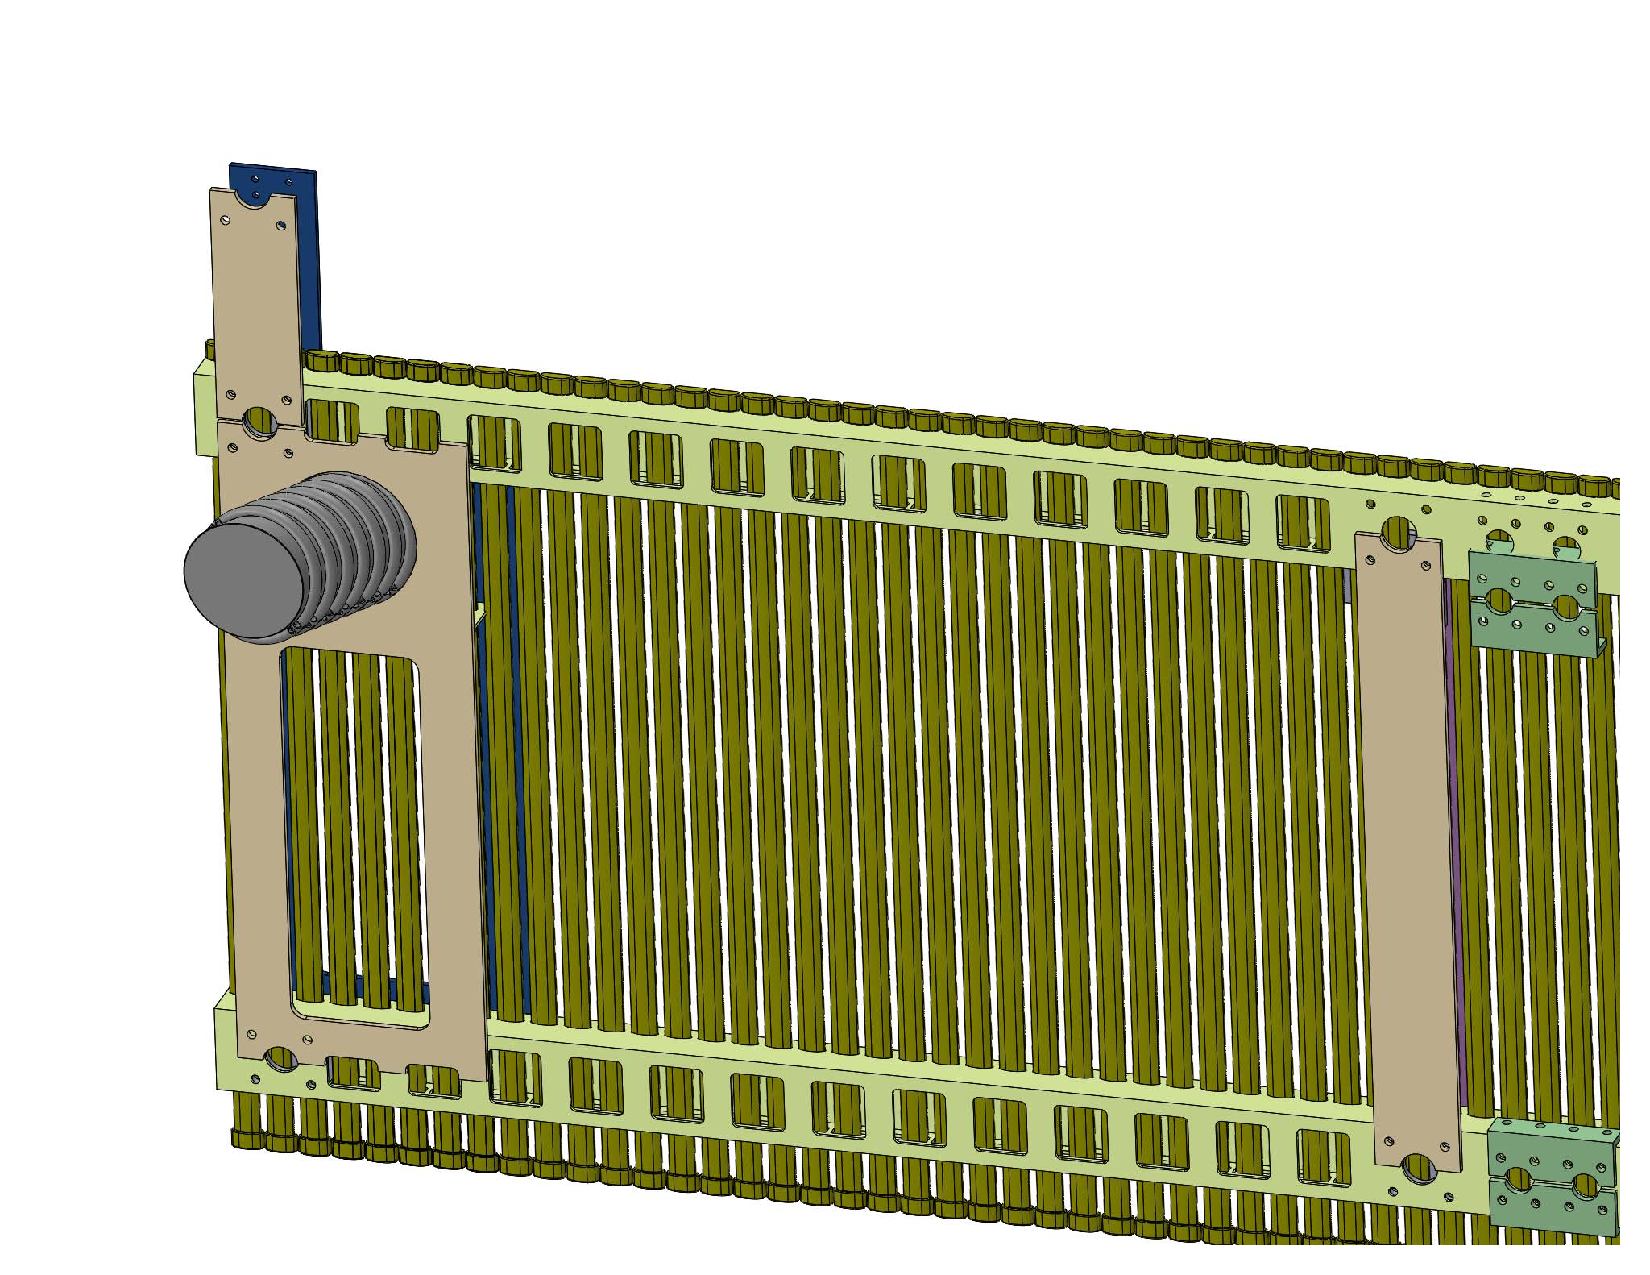
\includegraphics[width=0.75\linewidth]{beamplug-fc.pdf}
\end{cdrfigure}
\begin{cdrfigure}[Beam plug to CPA connection]{beamplug-fc2}{Cutaway sideview of the beam plug to field cage interface.}
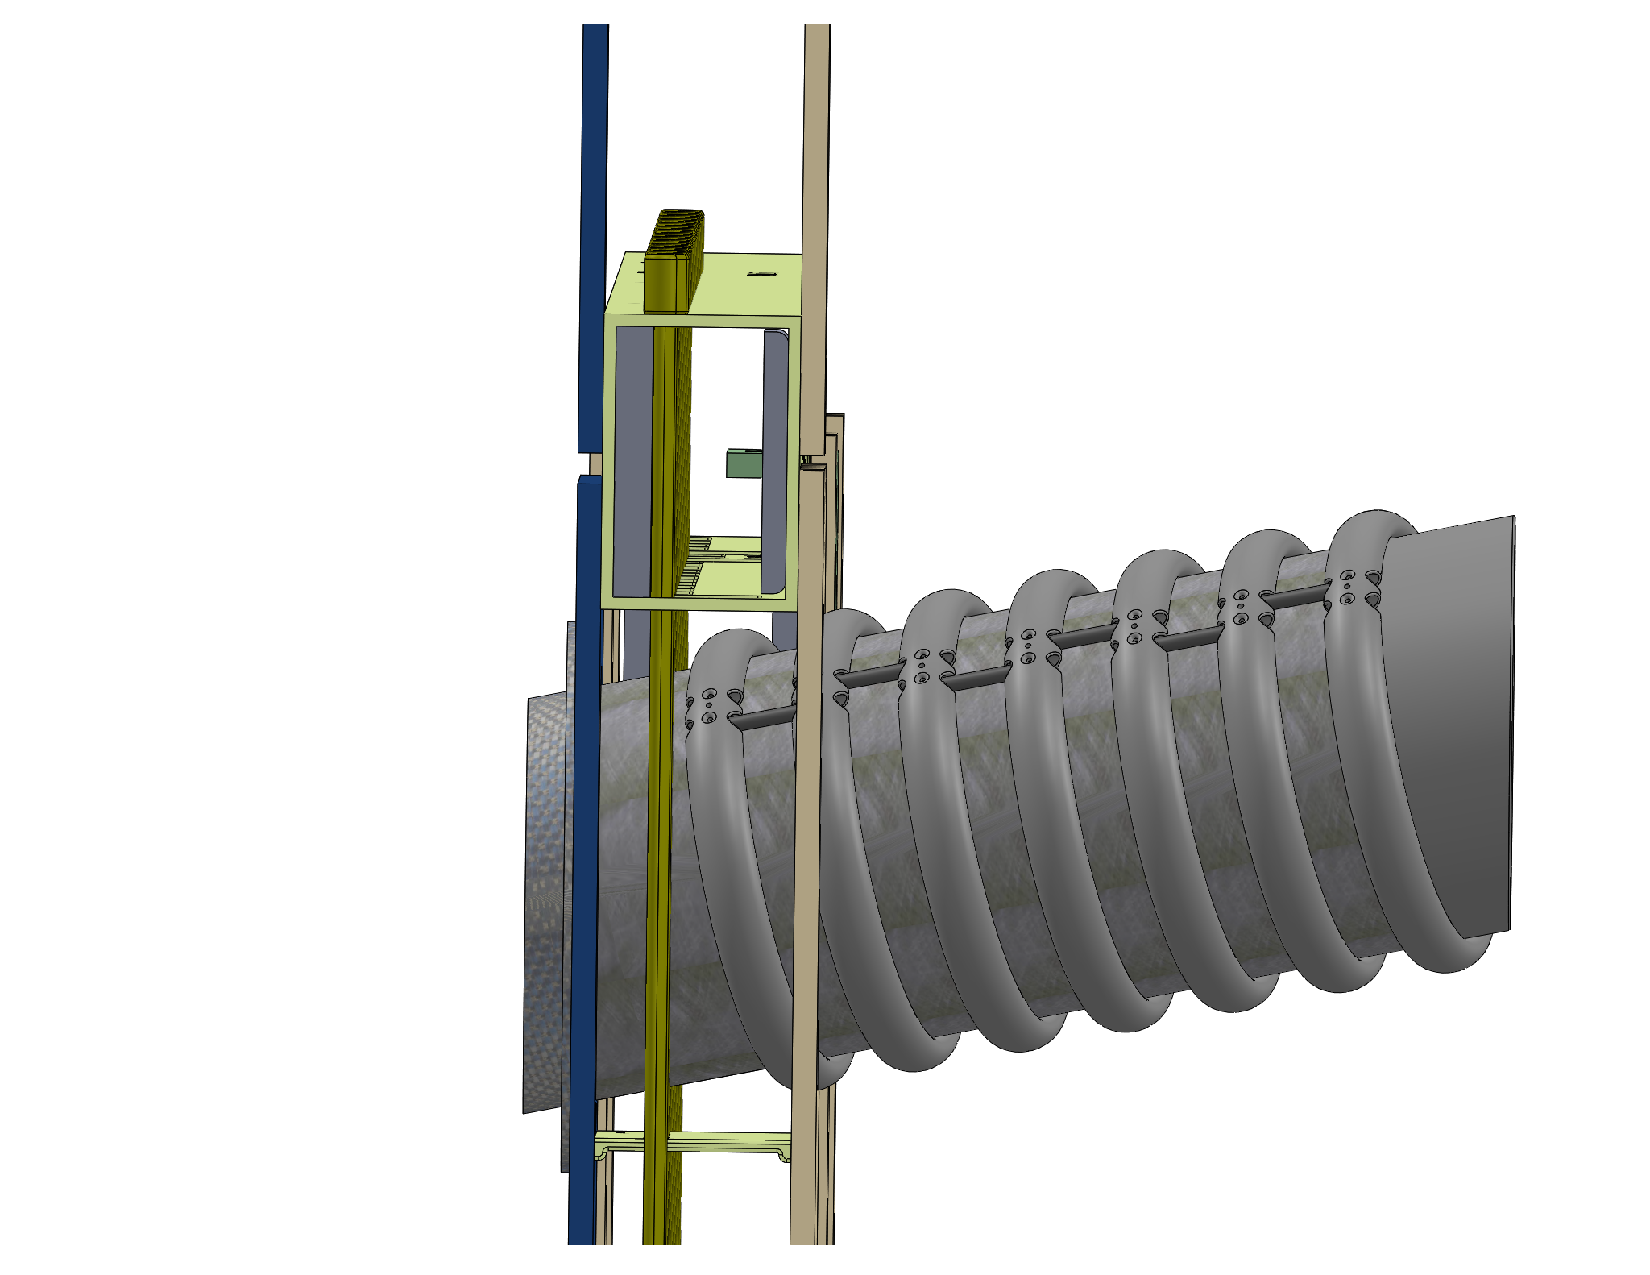
\includegraphics[width=0.5\linewidth]{beamplug-fc2.pdf}
\end{cdrfigure}
